\receta{Lomito Alcaparrado}
\index{lomito alcaparrado}

Rinde para 6 personas.

\begin{ingredientes}
\item  Preparación Lomo
\begin{itemize}
\item 1.5 kg de Lomo Viche
\item 4 Dientes de Ajo grandes
\item 1 Cucharada de Salsa Inglesa
\item Sal
\item Pimienta
\item Mantequilla para freír el lomo
\end{itemize}
\item Salsa:
\begin{itemize}
\item 30 g Mantequilla
\item 75 g Harina de trigo
\item 1 Cubo de caldo de carne
\item 2 Tazas de Agua
\item 200 g Alcaparras 
\item 150 g uvas pasas
\item Sal
\item Pimienta
\end{itemize}

\end{ingredientes}
\preparacion
Con 1 dia de anticipación, procesar finamente el ajo hasta obtener una pasta para adobar el lomo acompañado con la salsa inglesa, sal y pimienta.\\

En el momento de la preparación derretir la mantequilla en una sartén y freir el lomo por ambos lados.\\

En la misma sartén donde se doró la carne, colocar los 30 g de Mantequilla y dejarla derretir,  incorporar poco a poco la harina y el cuo de caldo. Verter el agua y revolver continuamente.Agregar las alcaparras y las uvas pasas, salpimentar si es necesario. Dejar hervir hasta que las mezcla espese.\\

Colocar en una refractaria el lomo y bañarlo con esta salsa. Llevar al horno precalentado a $350^\circ$F ($177^\circ$C) durante $\rfrac{1}{2}$ hora.

\begin{center}
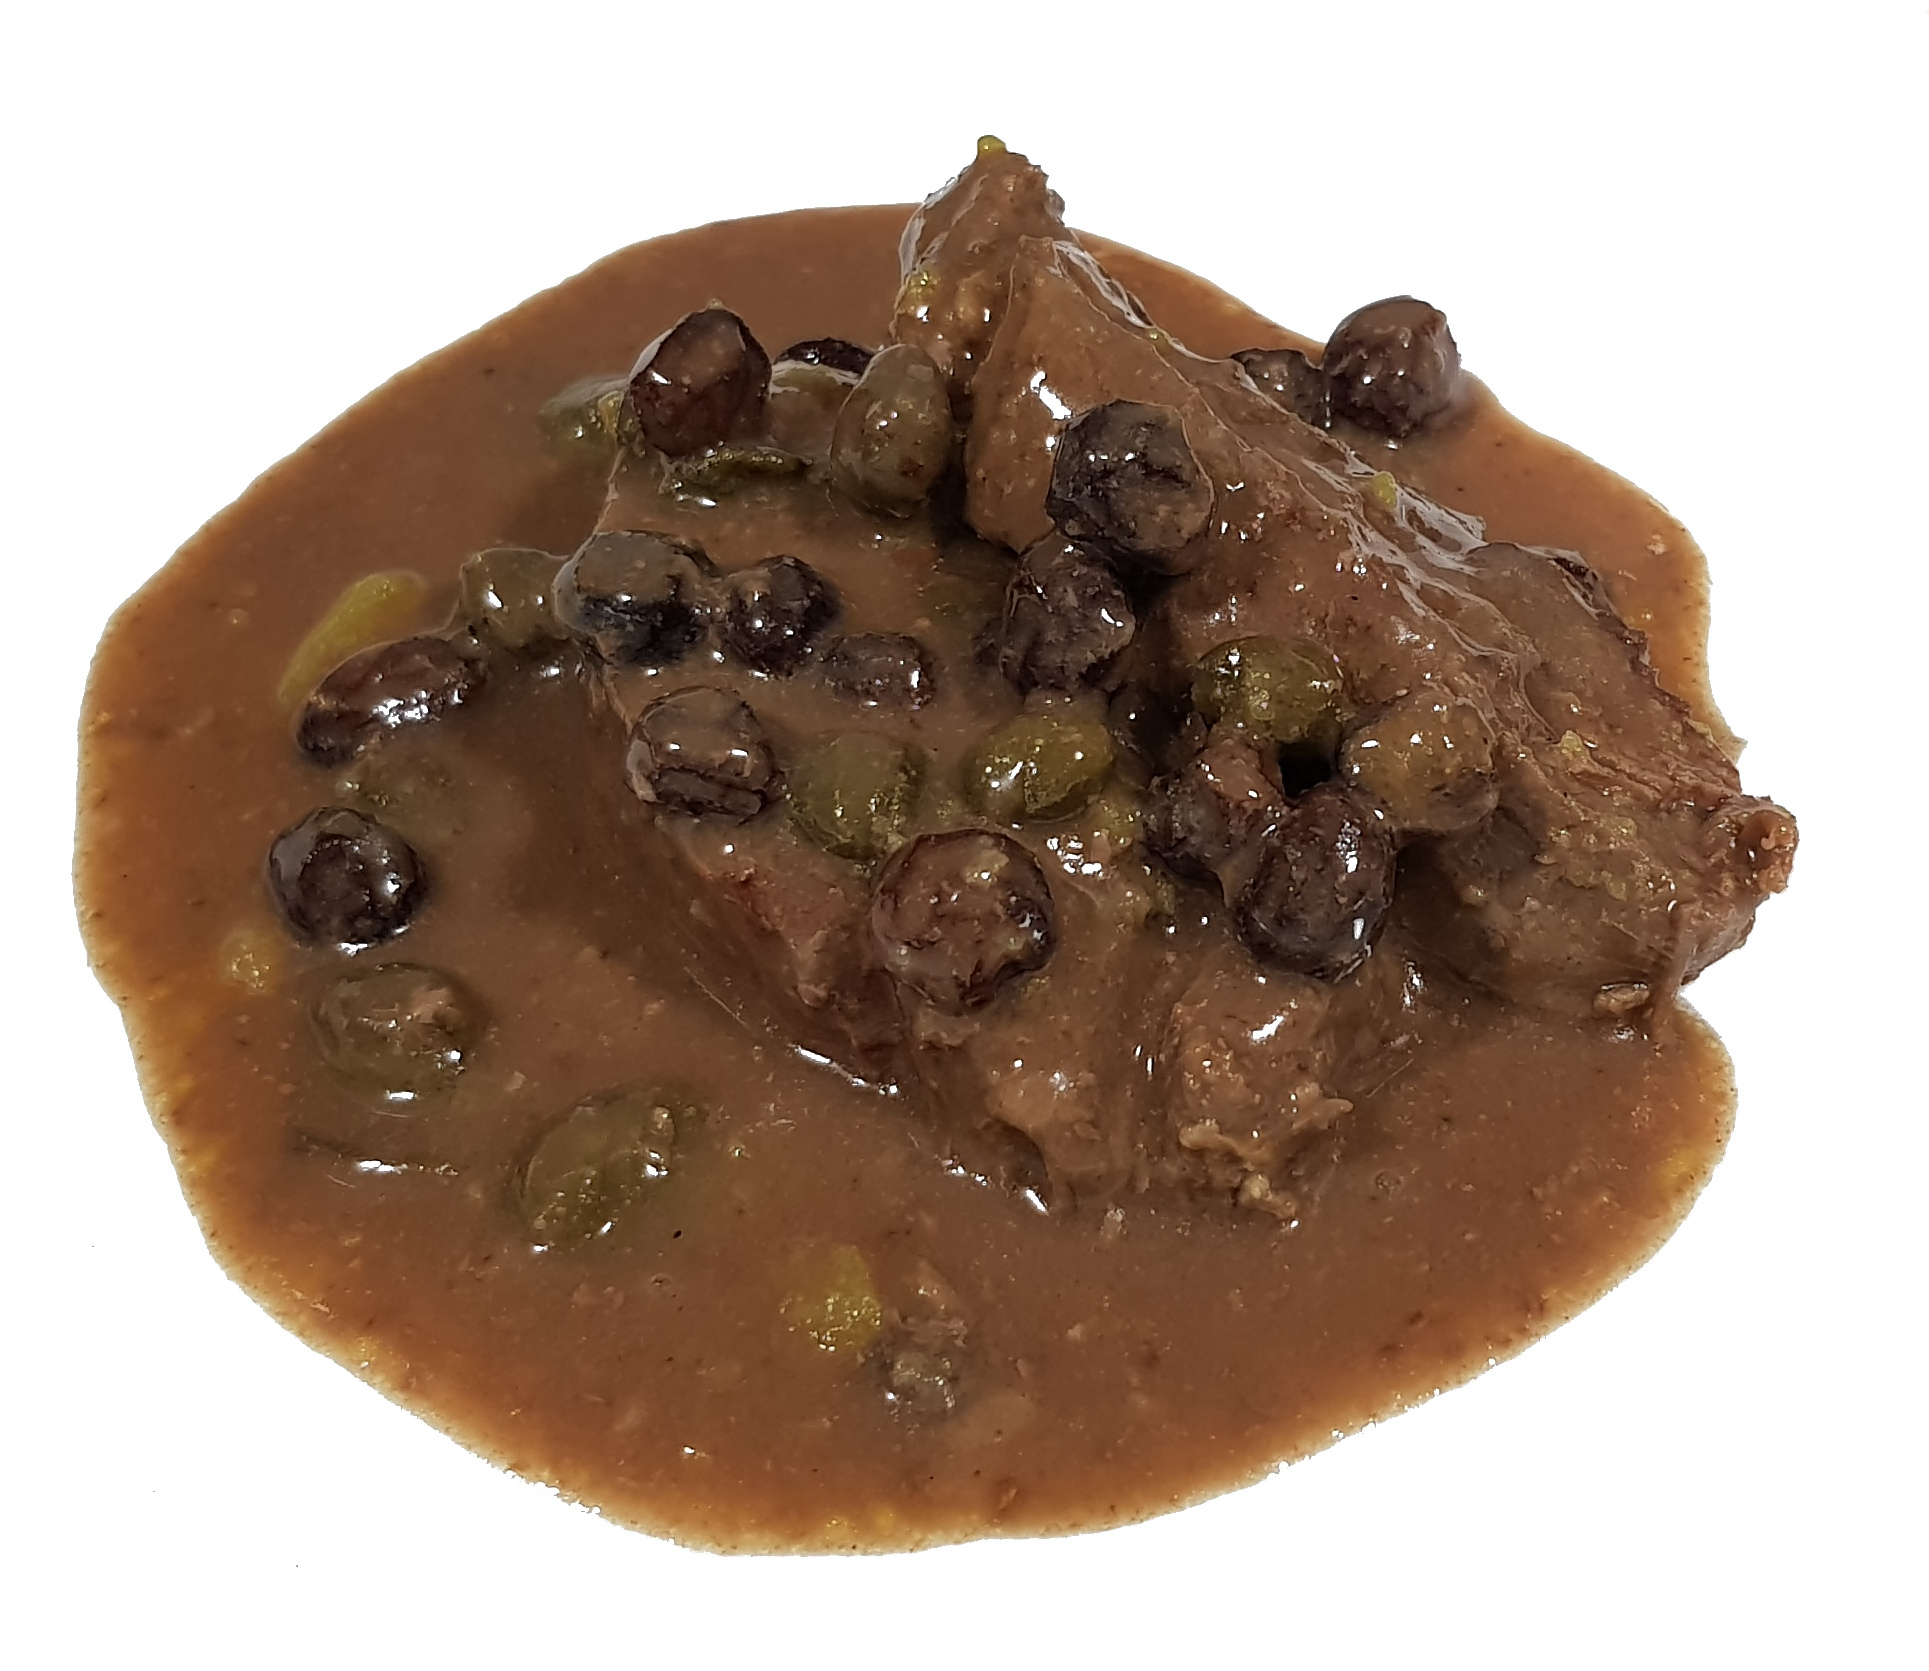
\includegraphics[width=0.8\textwidth]{fotos/lomito_alcaparrado.jpg}
\end{center}